% $Id: appendix.tex 1793 2016-01-18 18:18:16Z lv39 $
\appendix
\section*{Appendix}
%\clearpage
\section*{Ramp algorithm in SAS}
\lstinputlisting{rampdist.sas}

\clearpage
\section*{Tables}

\begin{table}
\caption{Suppressions in establishment-level BDS\label{tab:bds_e}}
\centering
\begin{tabular}{|l|r|rrr|}\hline%
               &                 \bfseries Number &\multicolumn{3}{c|}{\bfseries Suppressions (\%)}\\
\cline{3-5}
\bfseries Type  &\bfseries of     &                            & \multicolumn{2}{c|}{\bfseries Job creation}\\
\cline{4-5}
                                                          &\bfseries  cells& \bfseries Any  &\bfseries by entrants &\bfseries 
                                                          by continuers\\
\hline
\csvreader[head to column names,late after line=\\,late after last line=\\\hline]%
{programs/bds_e_suppressions_multi.csv}{}%
{\typename &  \cells & \percentsup  & \jcbirths &\jcconts}%
\multicolumn{4}{p{0.6\textwidth}}{\footnotesize Note: Cells are year $x$ categories, where the 
number of categories varies by published table.}
\end{tabular}
\end{table}

\clearpage
\begin{table}[p]
		\setlength{\tabcolsep}{6pt}
\caption{Analytic validity: Feasibility of AR(2) regressions \label{tab:bds_e_pctmiss}}
\centering
%\begin{tabular}{|lc|r|rrr|}\hline%
\csvreader[tabular=|l|r|r|rrr|rrr|r|,table head=\hline 
	&Number 
	&\multicolumn{8}{c|}{Percent} 
\\
Variable 
	&feasible 
	& \multicolumn{8}{c|}{Infeasible}                
\\
    & $X_{k^\prime t}$ 
    & $X_{k^\prime t}^{(s)}$ 
    & $X_{k^\prime t}^{(0)}$ 
    & $X_{k^\prime t}^{(i)}$
    & $X_{k^\prime t}^{(in)}$
    & $X_{k^\prime t}^{(ii)}$
    & $X_{k^\prime t}^{(iiw)}$
    & $X_{k^\prime t}^{(iin)}$
    & $X_{k^\prime t}^{(n)}$
    \\\hline,
	late after line=\\,late after last line=\\\hline]%
{results/r_e_agesz_all_missing.csv}{Variable=\V,number=\colz,missing1=\cola,missing2=\colb,missing3=\colc,missing4=\cold,missing5=\cole,missing6=\colf,missing7=\colg,missing8=\colh}%
{\V &  \colz & \cola & \colb & \colc & \cold & \cole & \colf & \colg &\colh}%
\end{table}

\clearpage
\begin{table}[p]
	\setlength{\tabcolsep}{6pt}
\caption{Analytic validity: AR(2) regressions with significant parameters\label{tab:bds_e_pctsign}}
\centering
%\begin{tabular}{|lc|r|rrr|}\hline%
\csvreader[tabular=|l|rr|rrr|rrr|r|,table head=\hline 
	& \multicolumn{9}{c|}{Percent} 
\\
Variable 
	& \multicolumn{9}{c|}{significant}
\\
    & $\rho_{1}$ 
    & $\rho_{1}^{(s)}$ 
    & $\rho_{1}^{(0)}$ 
    & $\rho_{1}^{(i)}$
    & $\rho_{1}^{(in)}$
    & $\rho_{1}^{(ii)}$
    & $\rho_{1}^{(iiw)}$
    & $\rho_{1}^{(iin)}$
    & $\rho_{1}^{(n)}$
    \\\hline,
	late after line=\\,late after last line=\\\hline]%
{results/r_e_agesz_all_significant.csv}{Variable=\V,significantconf2=\colz,significant1=\cola,significant2=\colb,significant3=\colc,significant4=\cold,significant5=\cole,significant6=\colf,significant7=\colg,significant8=\colh}%
{\V &  \colz & \cola & \colb & \colc & \cold & \cole & \colf & \colg &\colh }%
\end{table}


\clearpage
\begin{table}[p]
		\setlength{\tabcolsep}{6pt}
\caption{Analytic validity: AR(2) regressions: 
Coverage\label{tab:bds_e_coverage}}
\centering
%\begin{tabular}{|lc|r|rrr|}\hline%
\csvreader[tabular=|l|r|rrr|rrr|r|,table head=\hline 
	& \multicolumn{8}{c|}{} 
\\
Variable 
	& \multicolumn{8}{c|}{Coverage}
\\
    & $\rho_{1}^{(s)}$ 
    & $\rho_{1}^{(0)}$ 
    & $\rho_{1}^{(i)}$
    & $\rho_{1}^{(in)}$
    & $\rho_{1}^{(ii)}$
    & $\rho_{1}^{(iiw)}$
    & $\rho_{1}^{(iin)}$
    & $\rho_{1}^{(n)}$
    \\\hline,
	late after line=\\,late after last line=\\\hline]%
{results/r_e_agesz_all_coverage.csv}{Variable=\V,coverage1=\cola,coverage2=\colb,coverage3=\colc,coverage4=\cold,coverage5=\cole,coverage6=\colf,coverage7=\colg,coverage8=\colh}%
{\V &  \cola & \colb & \colc & \cold & \cole  & \colf & \colg &\colh}%
\end{table}

\clearpage
\begin{table}[p]
			\setlength{\tabcolsep}{6pt}
\caption{Analytic validity: AR(2) regressions: Interval 
overlap\label{tab:bds_e_jk}}
\centering
%\begin{tabular}{|lc|r|rrr|}\hline%
\csvreader[tabular=|l|r|rrr|rrr|r|,table head=\hline 
	& \multicolumn{8}{c|}{Interval} 
\\
Variable 
	& \multicolumn{8}{c|}{overlap}
\\
    & $J_k^{(s)}$ 
    & $J_k^{(0)}$ 
    & $J_k^{(i)}$
    & $J_k^{(in)}$
    & $J_k^{(ii)}$
    & $J_k^{(iiw)}$
    & $J_k^{(iin)}$
    & $J_k^{(n)}$
    \\\hline,
	late after line=\\,late after last line=\\\hline]%
{../results/r_e_agesz_all_Jk.csv}{Variable=\V,Jk1=\cola,Jk2=\colb,Jk3=\colc,Jk4=\cold,Jk5=\cole,Jk6=\colf,Jk7=\colg,Jk8=\colh}%
{\V &  \cola & \colb & \colc & \cold & \cole & \colf & \colg &\colh}%
\end{table}


\clearpage
\begin{table}[p]
\caption{Suppressions in firm-level BDS\label{tab:bds_f}}
\centering
\begin{tabular}{lcrr}\hline%
&&\bfseries No. of&\bfseries Percent\\
\bfseries Type & \bfseries Level & \bfseries  cells
& \bfseries  suppressed\\
\hline
\\
\csvreader[head to column names]%
{programs/bds_f_suppressions.csv}{}%
{\type & \level & \cells & \percentsup\\}%
\\\hline
\multicolumn{4}{p{0.5\textwidth}}{\footnotesize Note: Cells are year $x$ categories, where the 
number of categories varies by published table.}

\end{tabular}
\end{table}

\clearpage
\section*{Figures}

\begin{figure}[h!]
	\centering
	\caption{Empirical distribution of noise\label{fig:fuzzgraph}}
	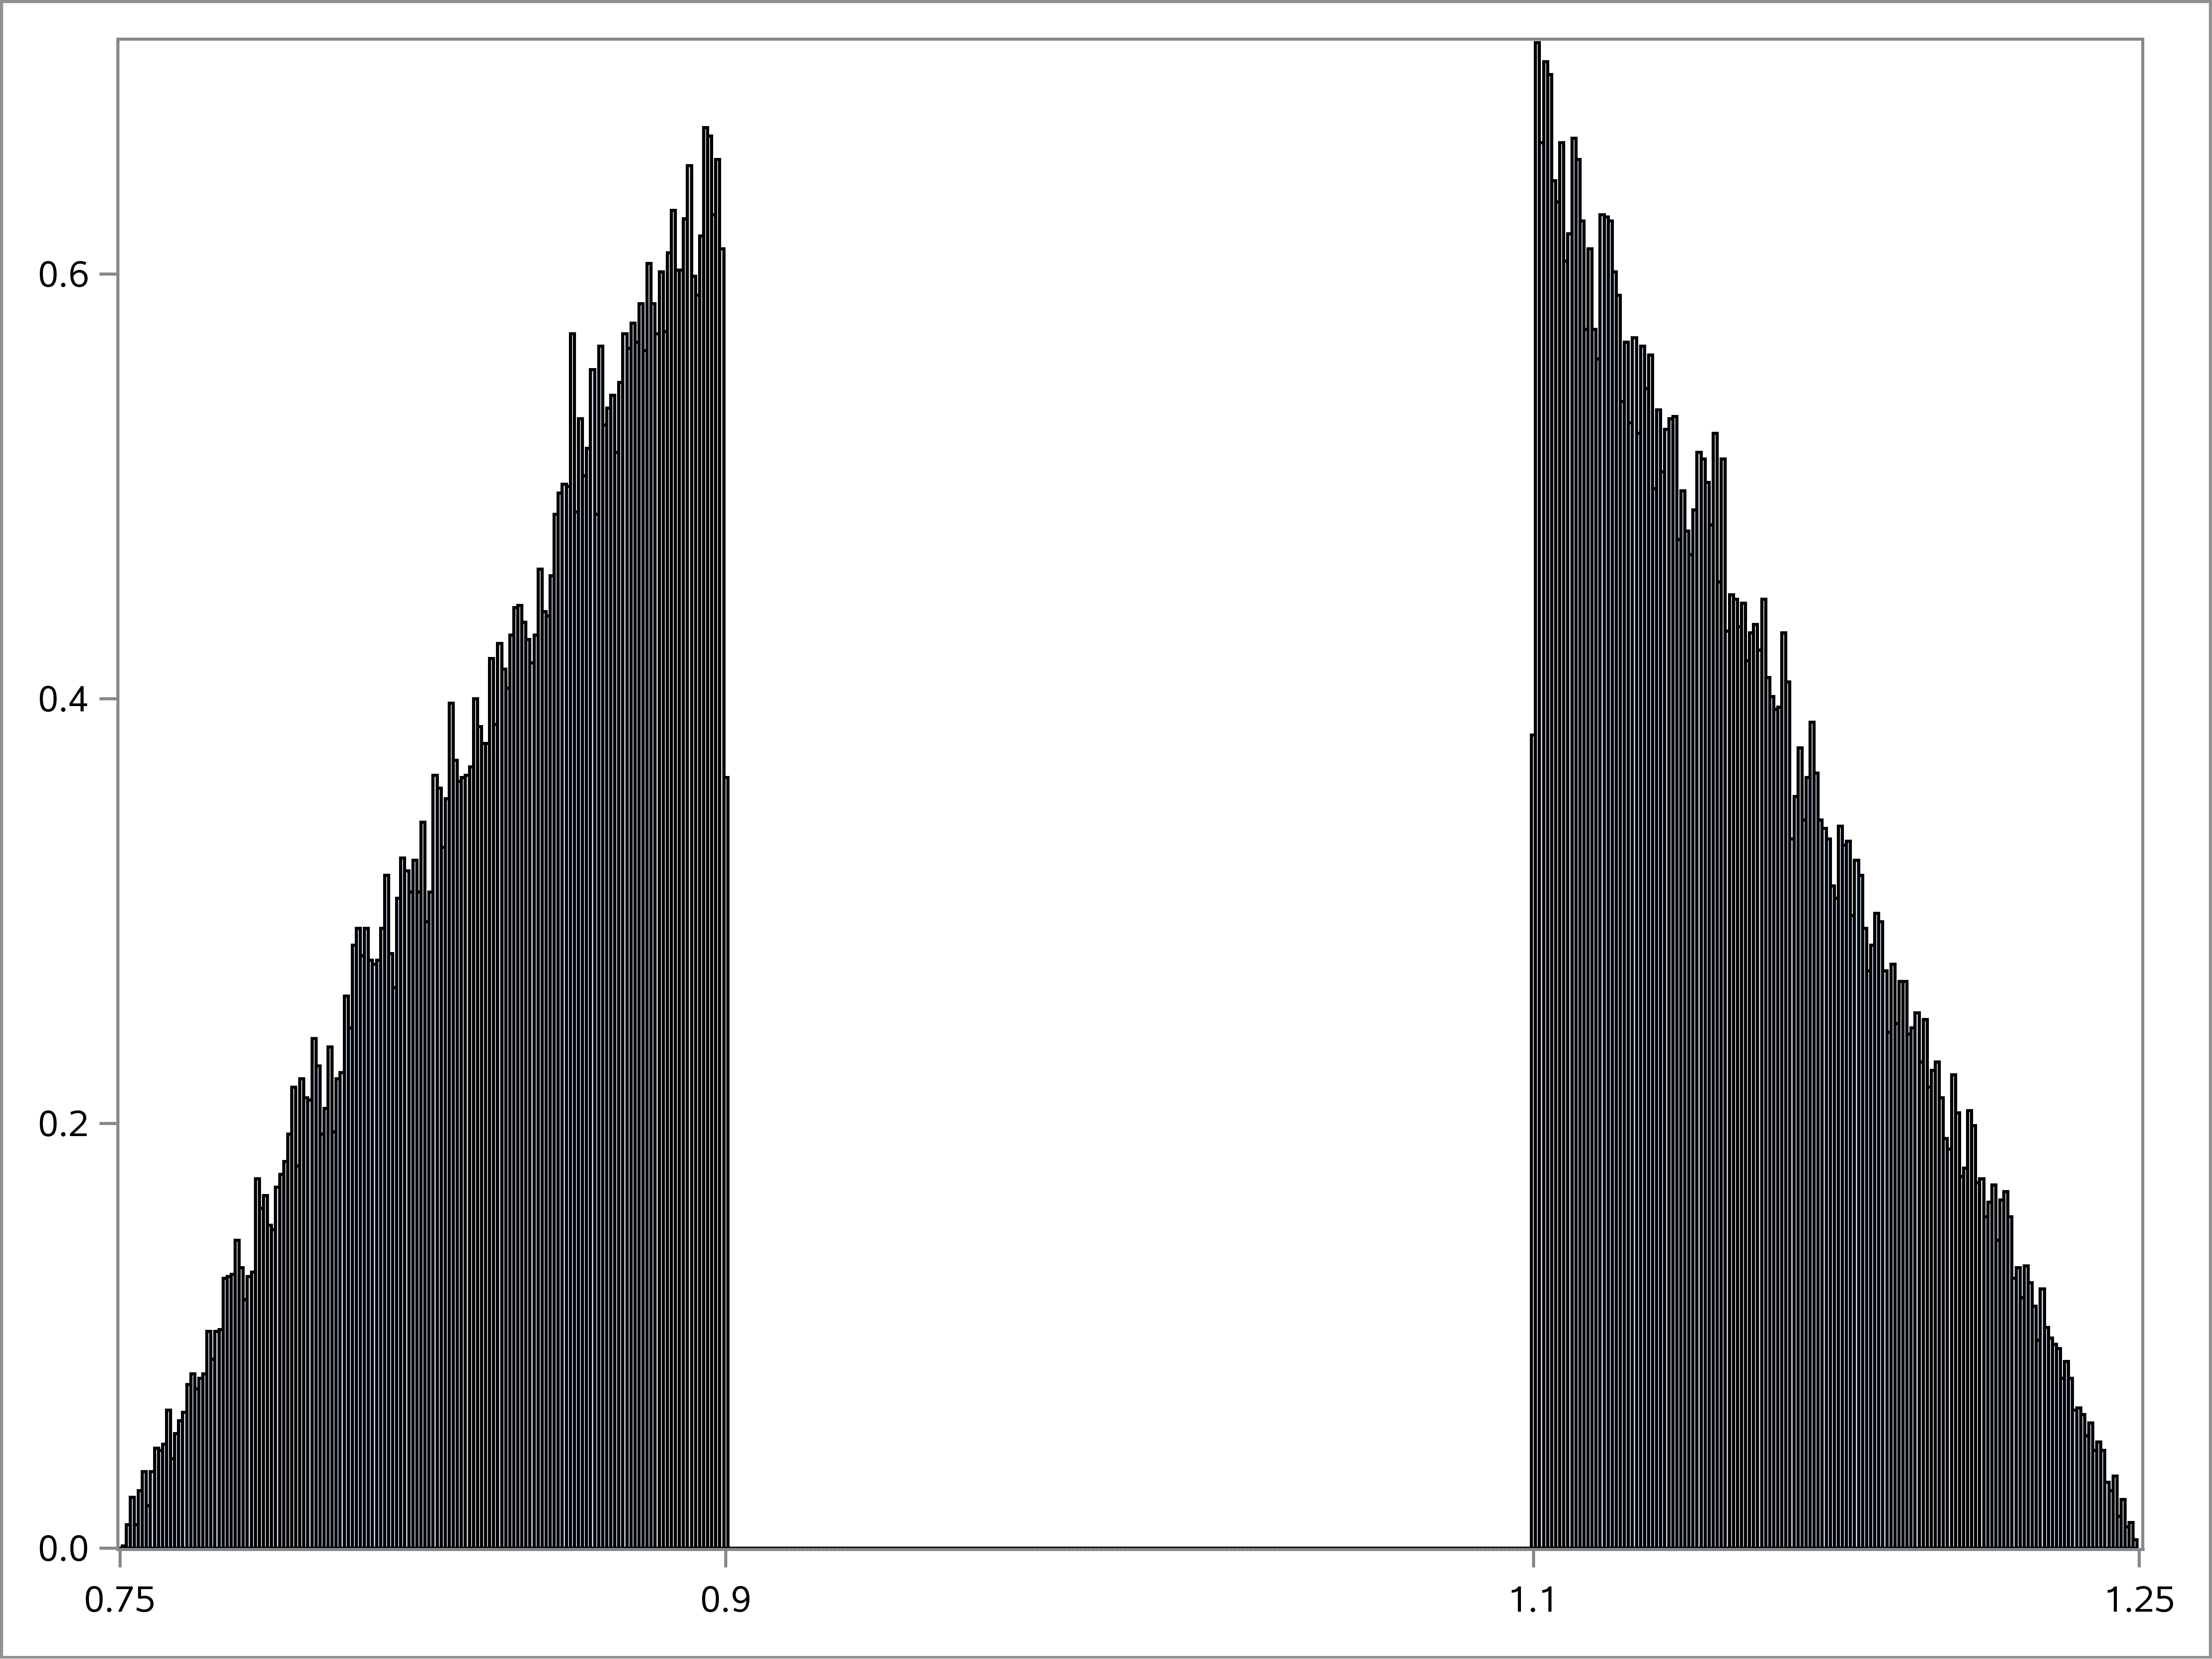
\includegraphics[width=0.9\textwidth]{SGPlotHiDef.png}
\end{figure}

\clearpage
\begin{figure}[p]
	\centering
	\caption{Levels of released and synthetic data\label{fig:level_denom}}
	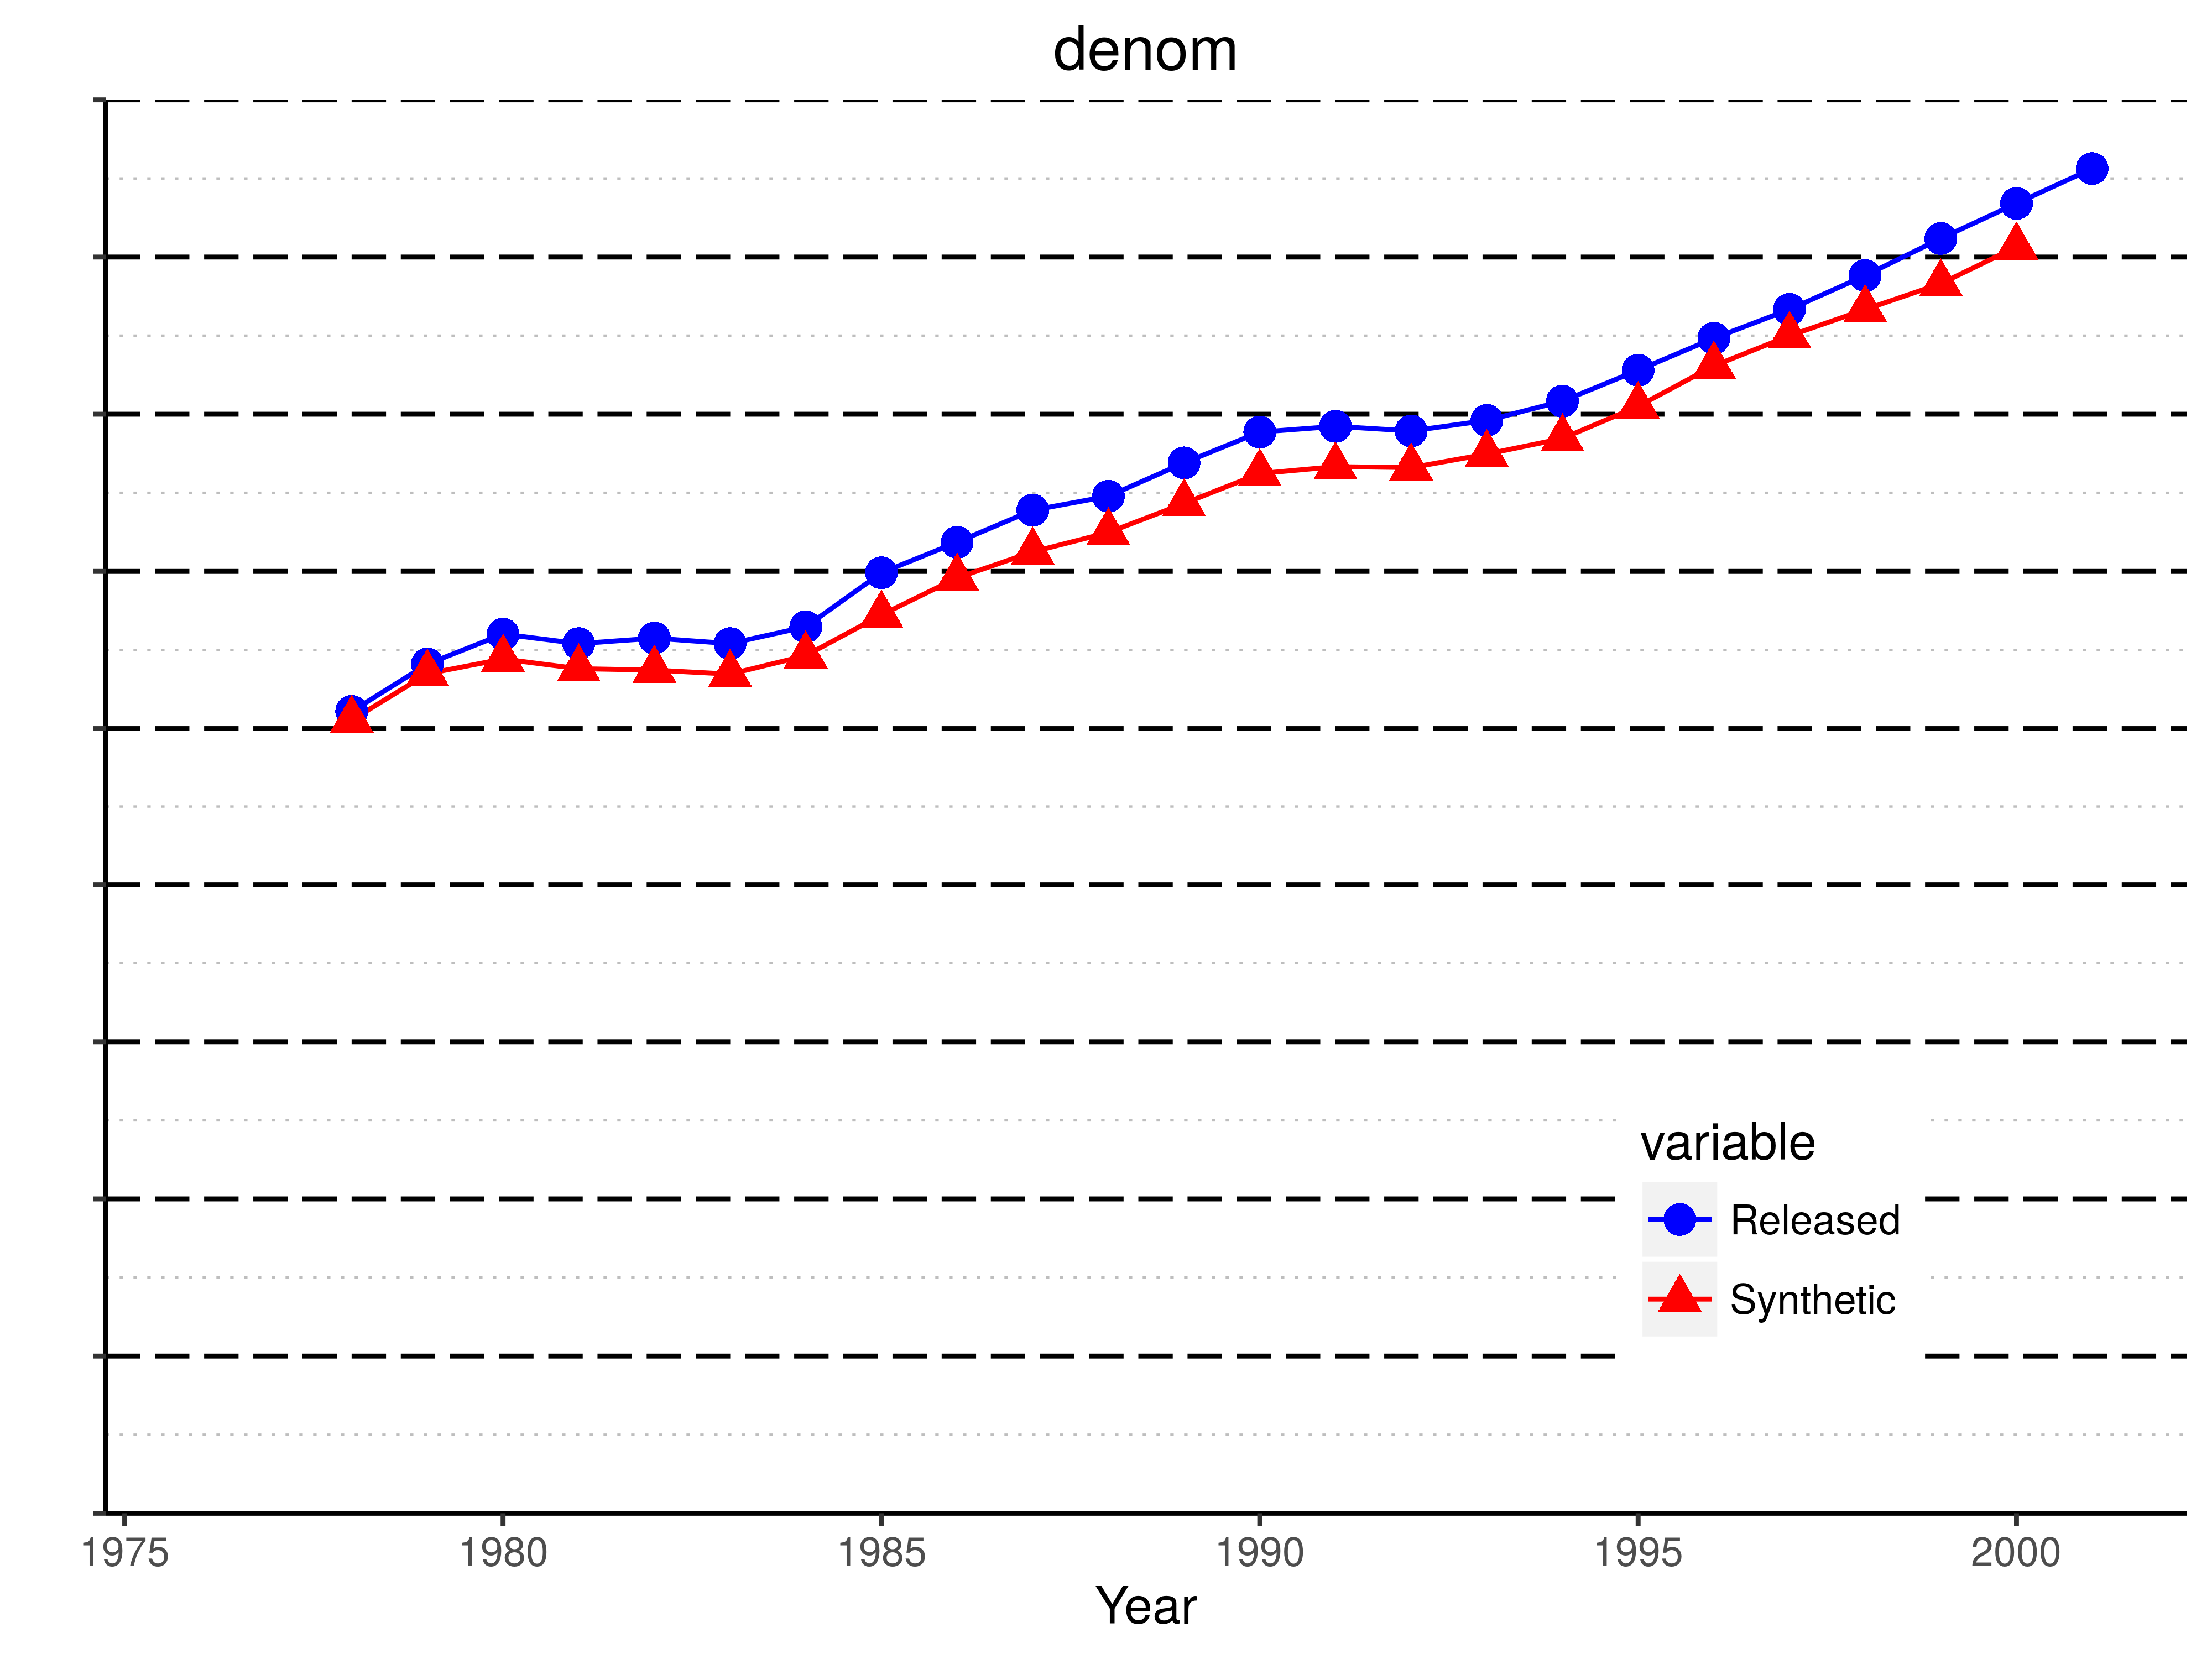
\includegraphics[width=0.45\textwidth]{results/graph_bds_real_vs_syn_denom_R}
	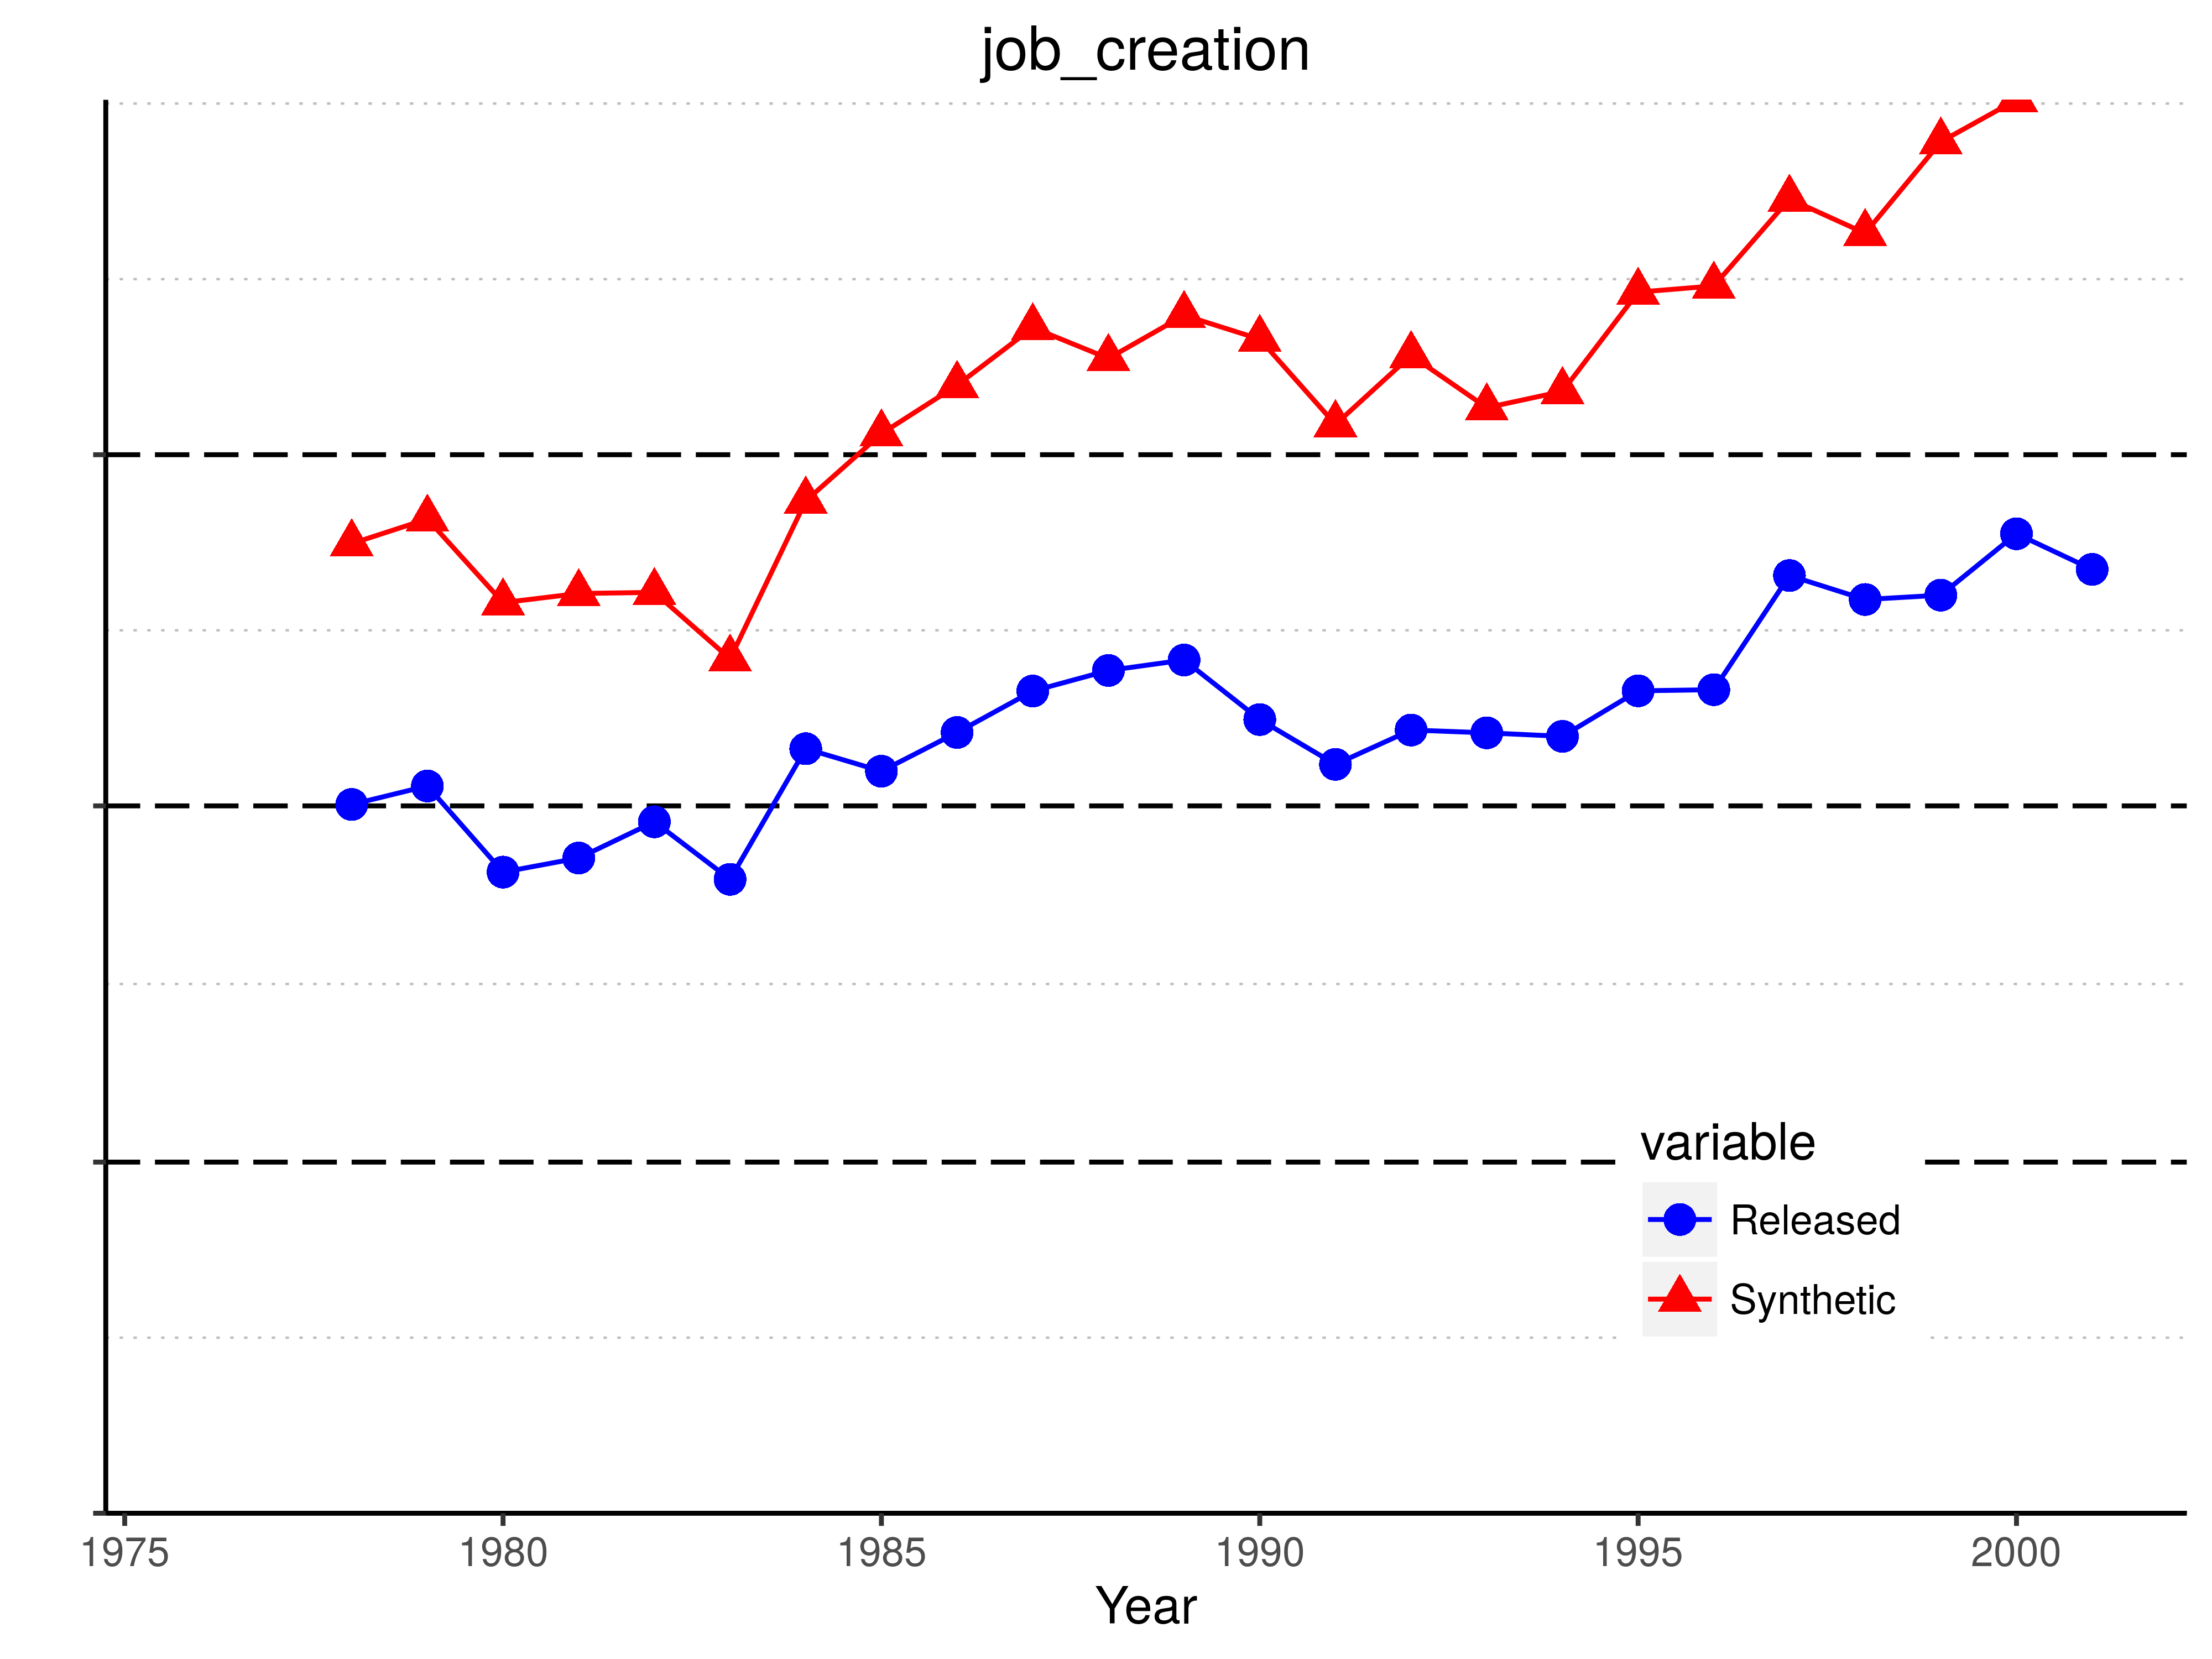
\includegraphics[width=0.45\textwidth]{results/graph_bds_real_vs_syn_job_creation_R}
	
	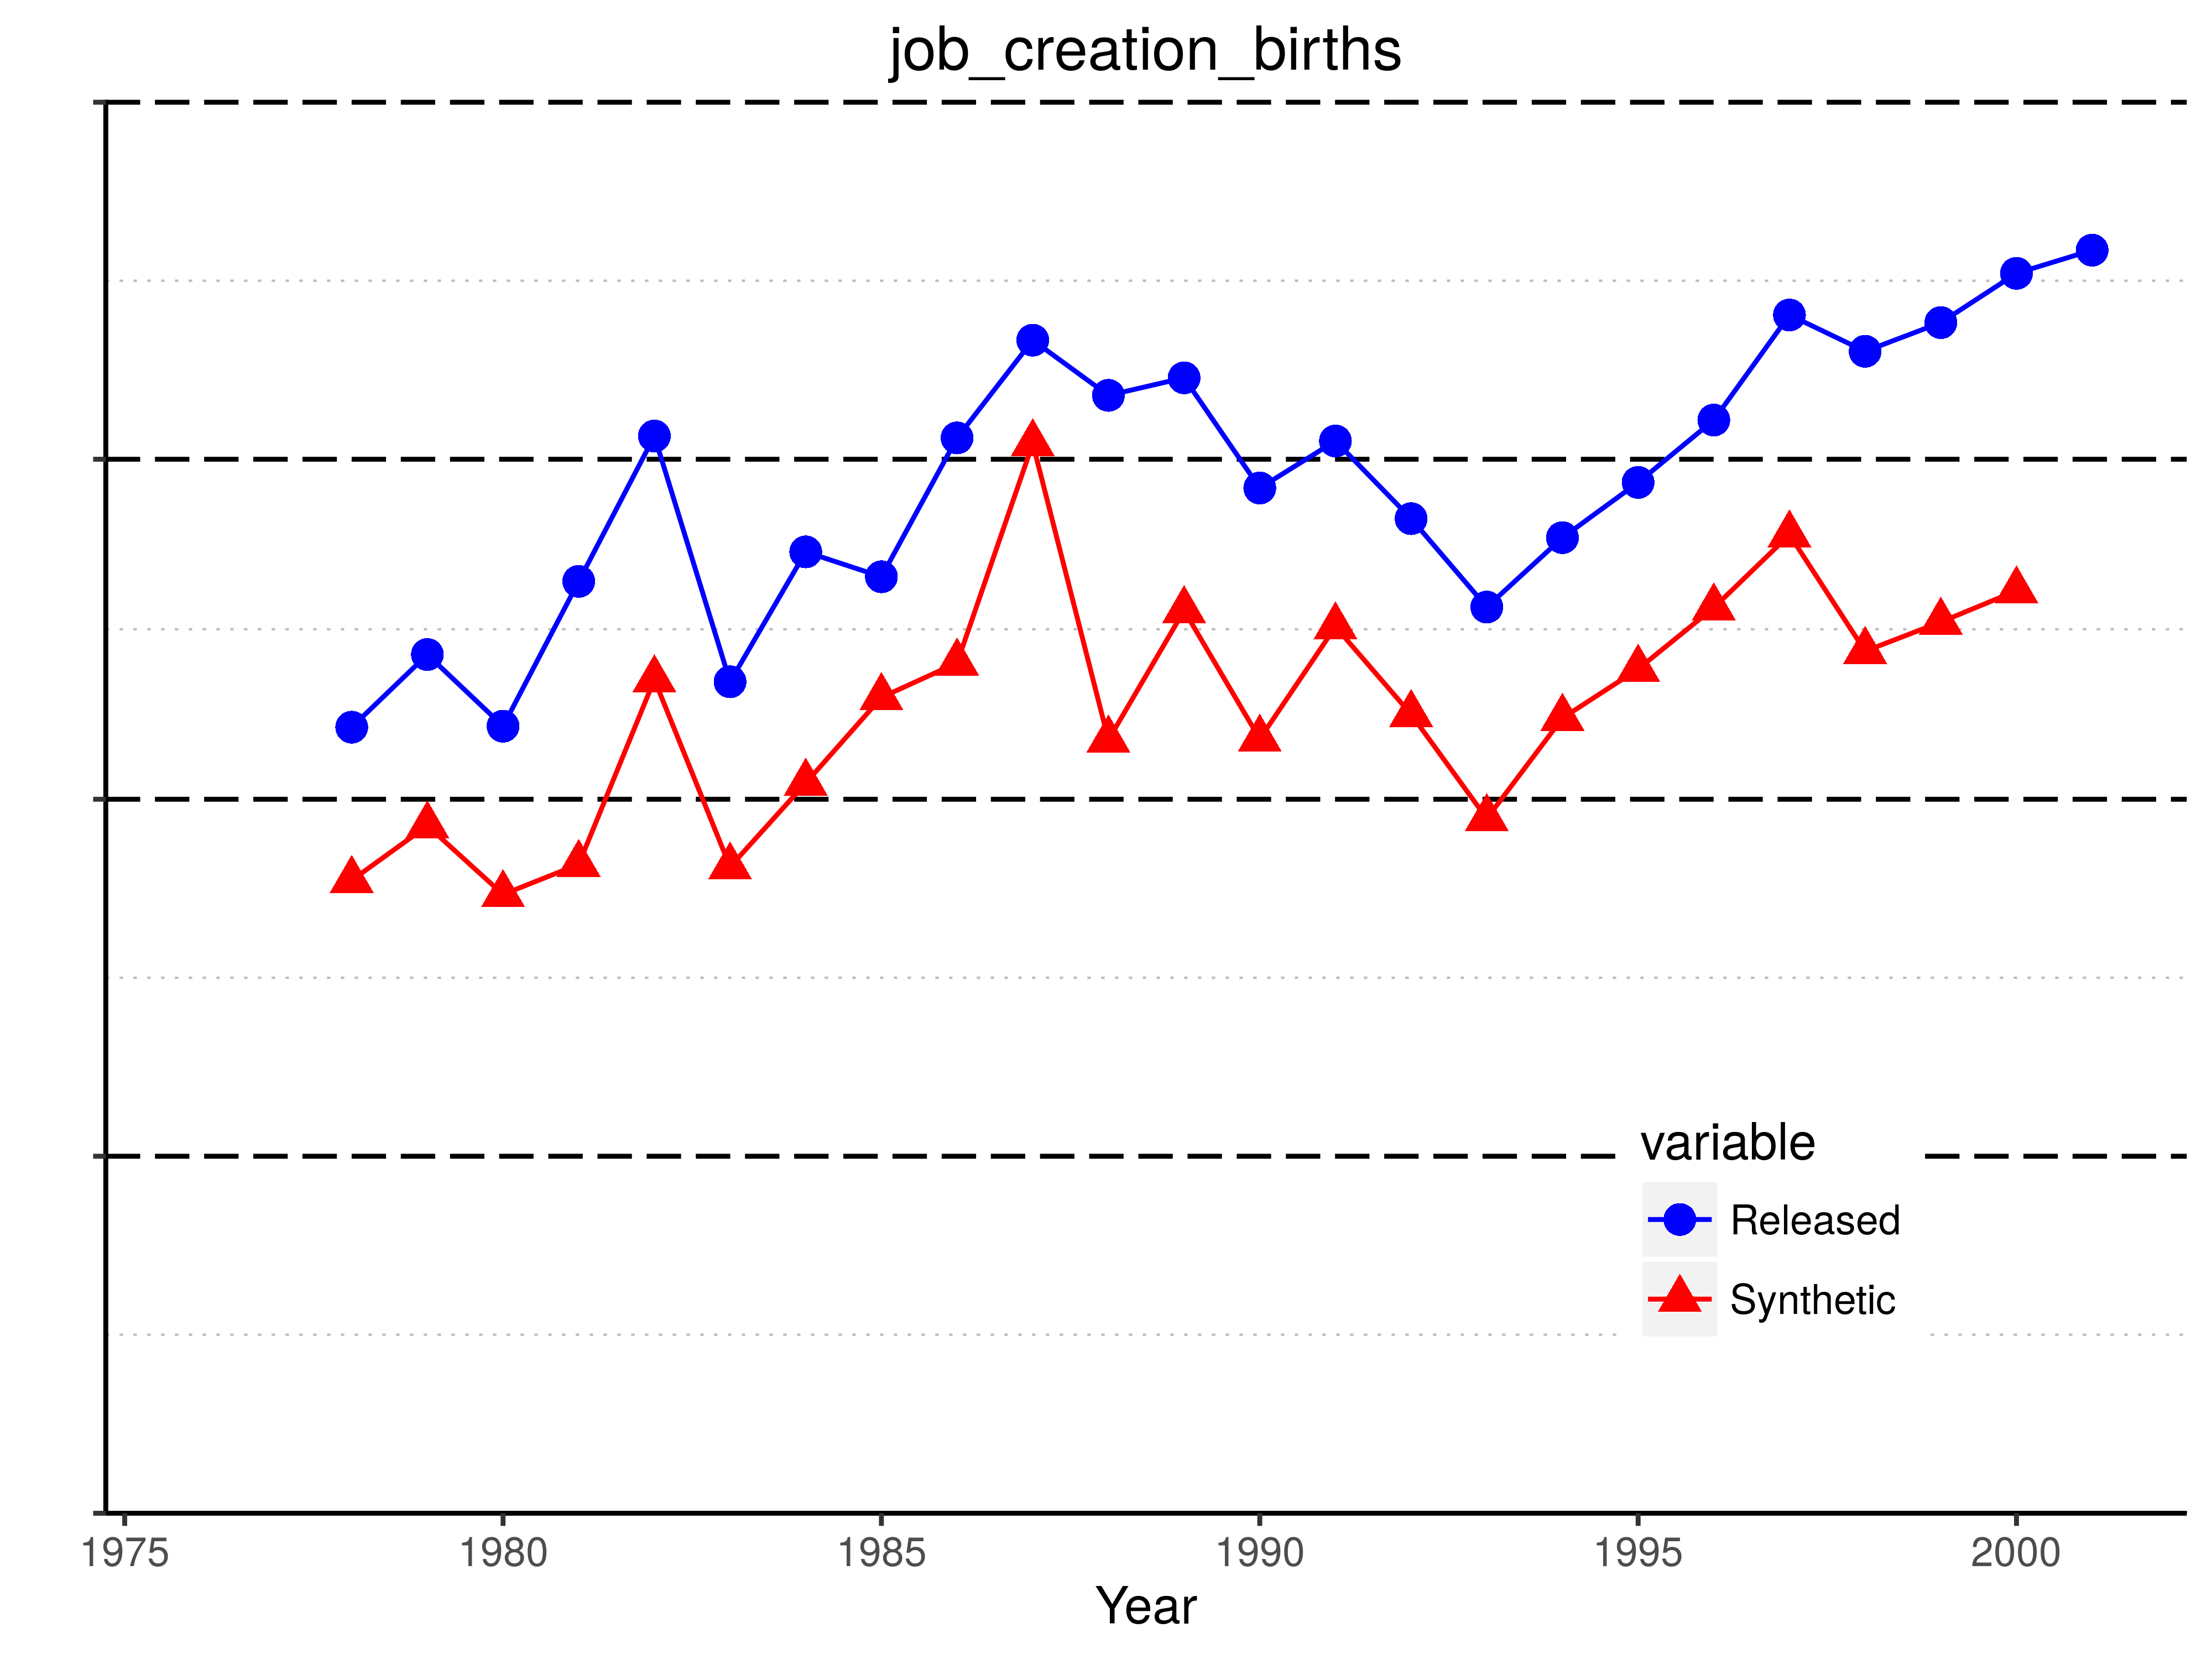
\includegraphics[width=0.45\textwidth]{results/graph_bds_real_vs_syn_job_creation_births_R}
	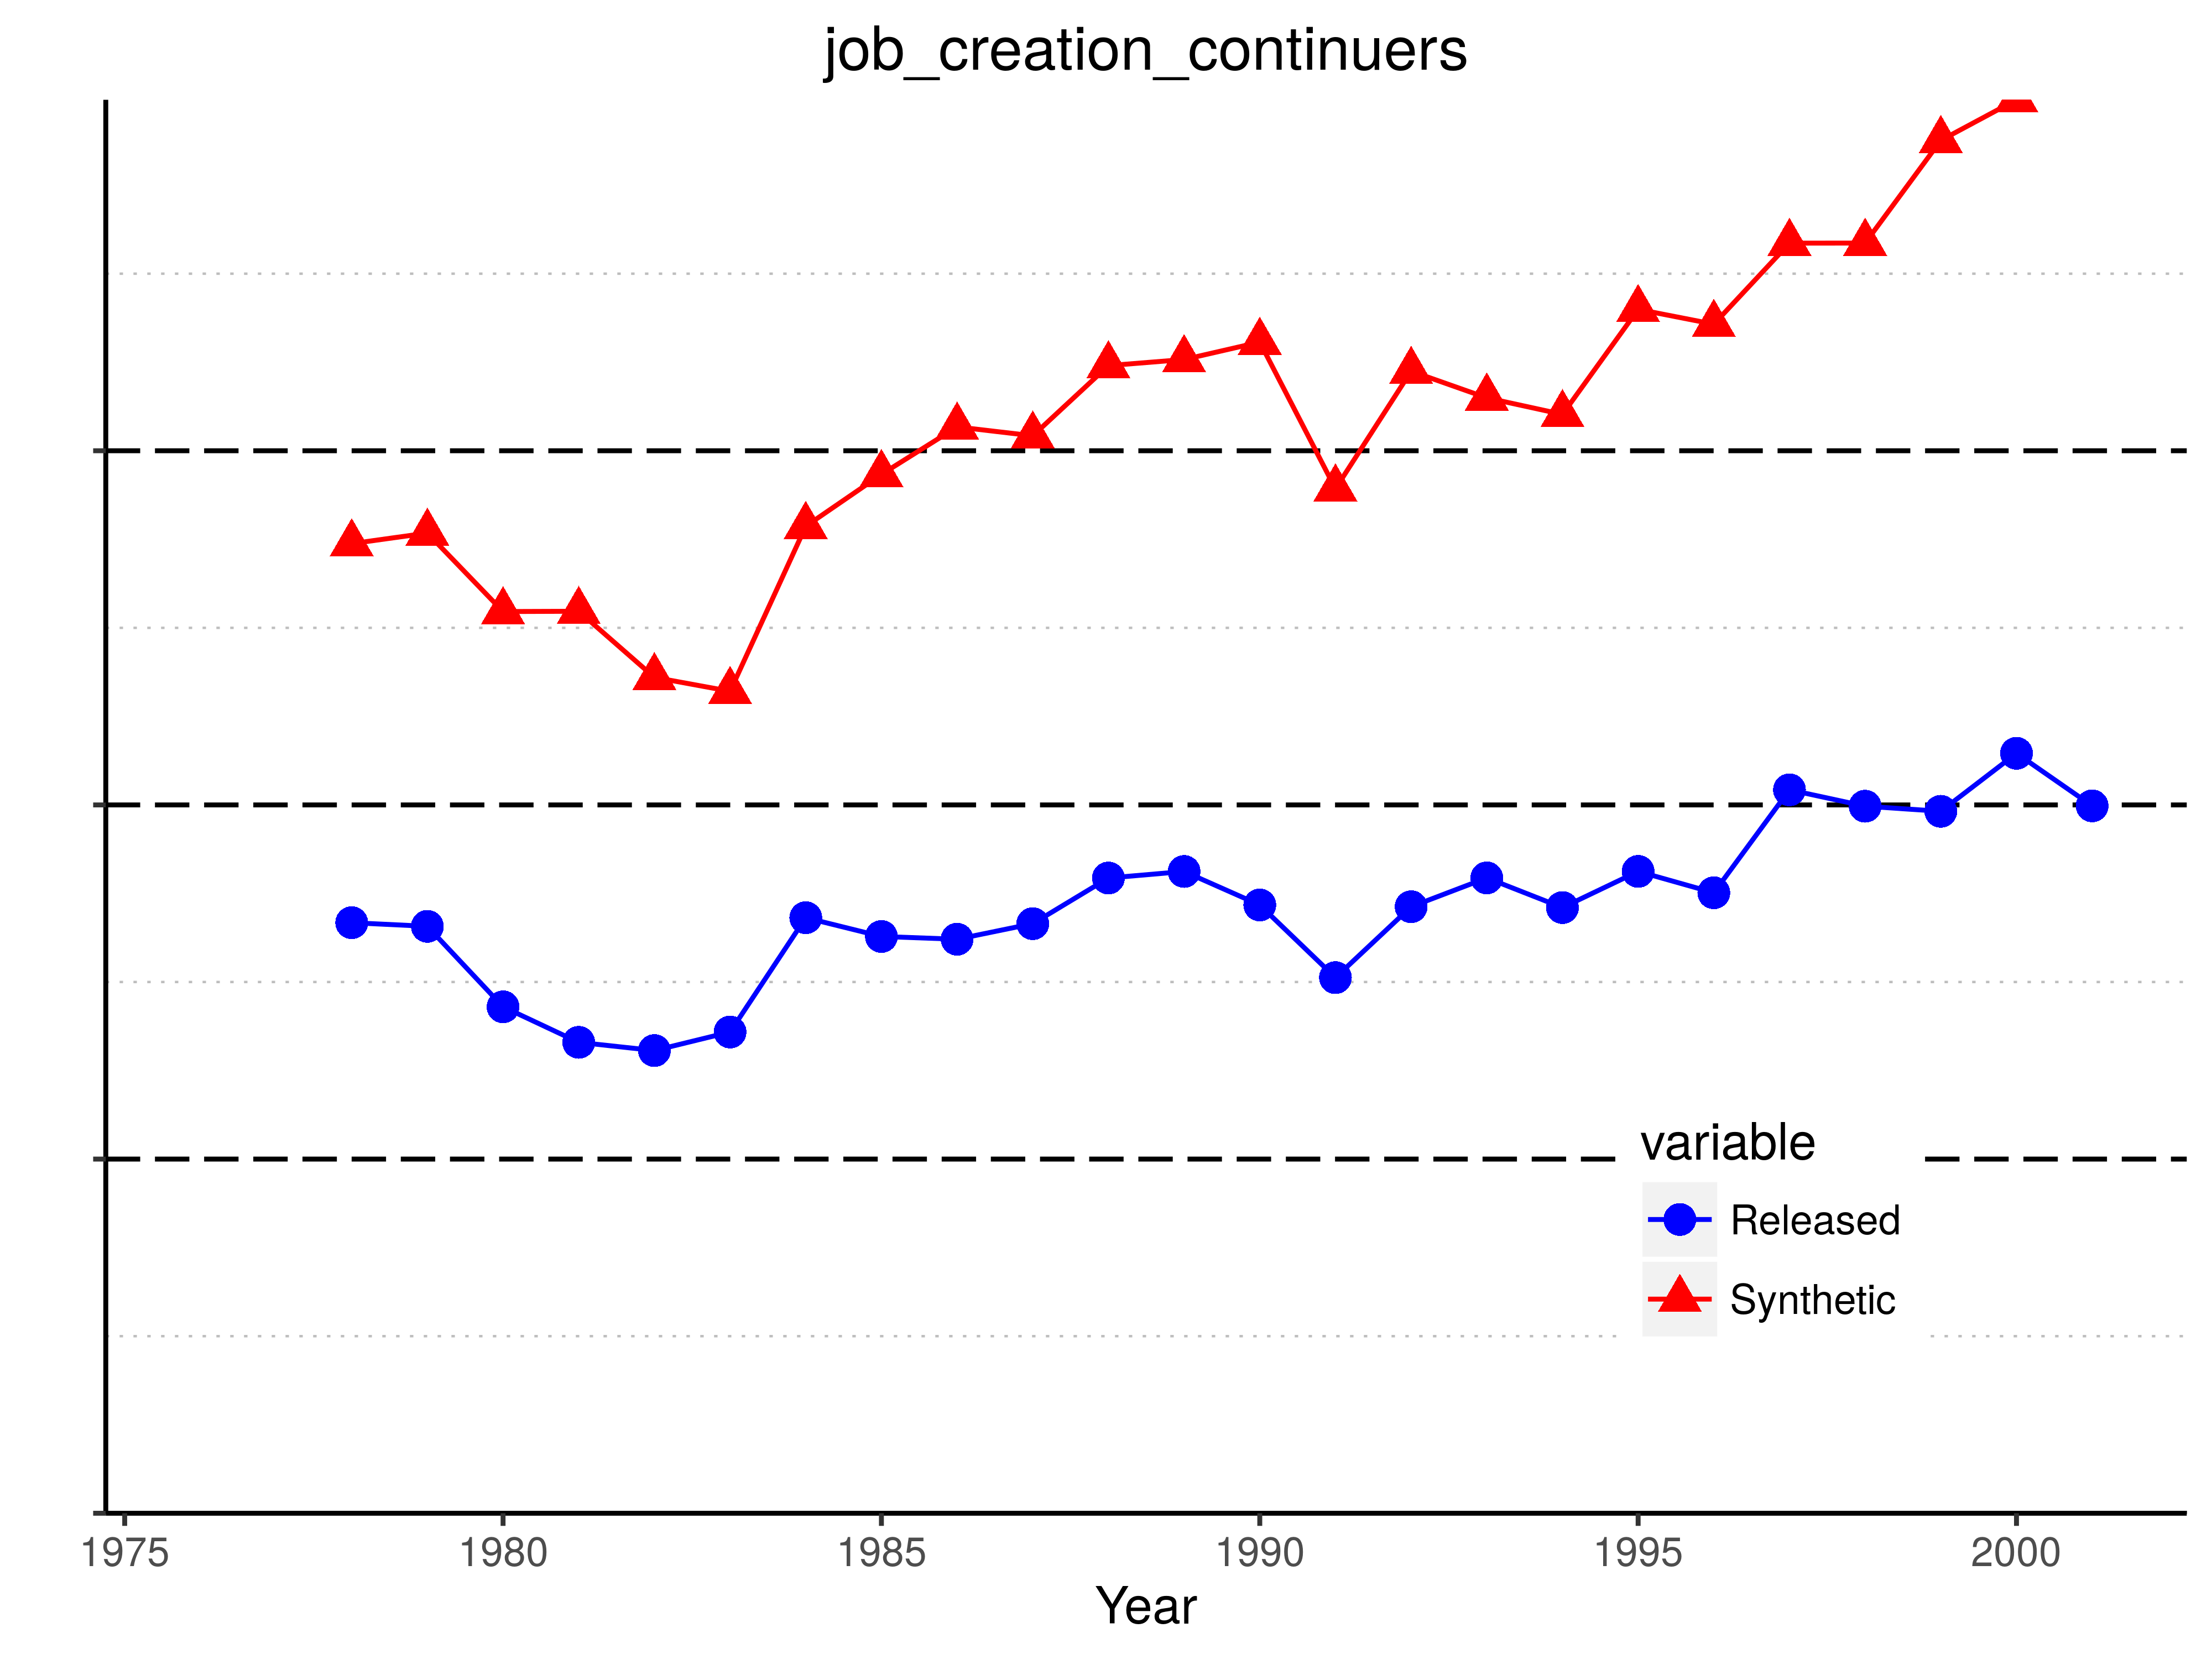
\includegraphics[width=0.45\textwidth]{results/graph_bds_real_vs_syn_job_creation_continuers_R}
\end{figure}

\clearpage
\begin{figure}[p]
\centering
\caption{Differences between released and synthetic data\label{fig:pct_denom}\label{fig:pct_jc}}
%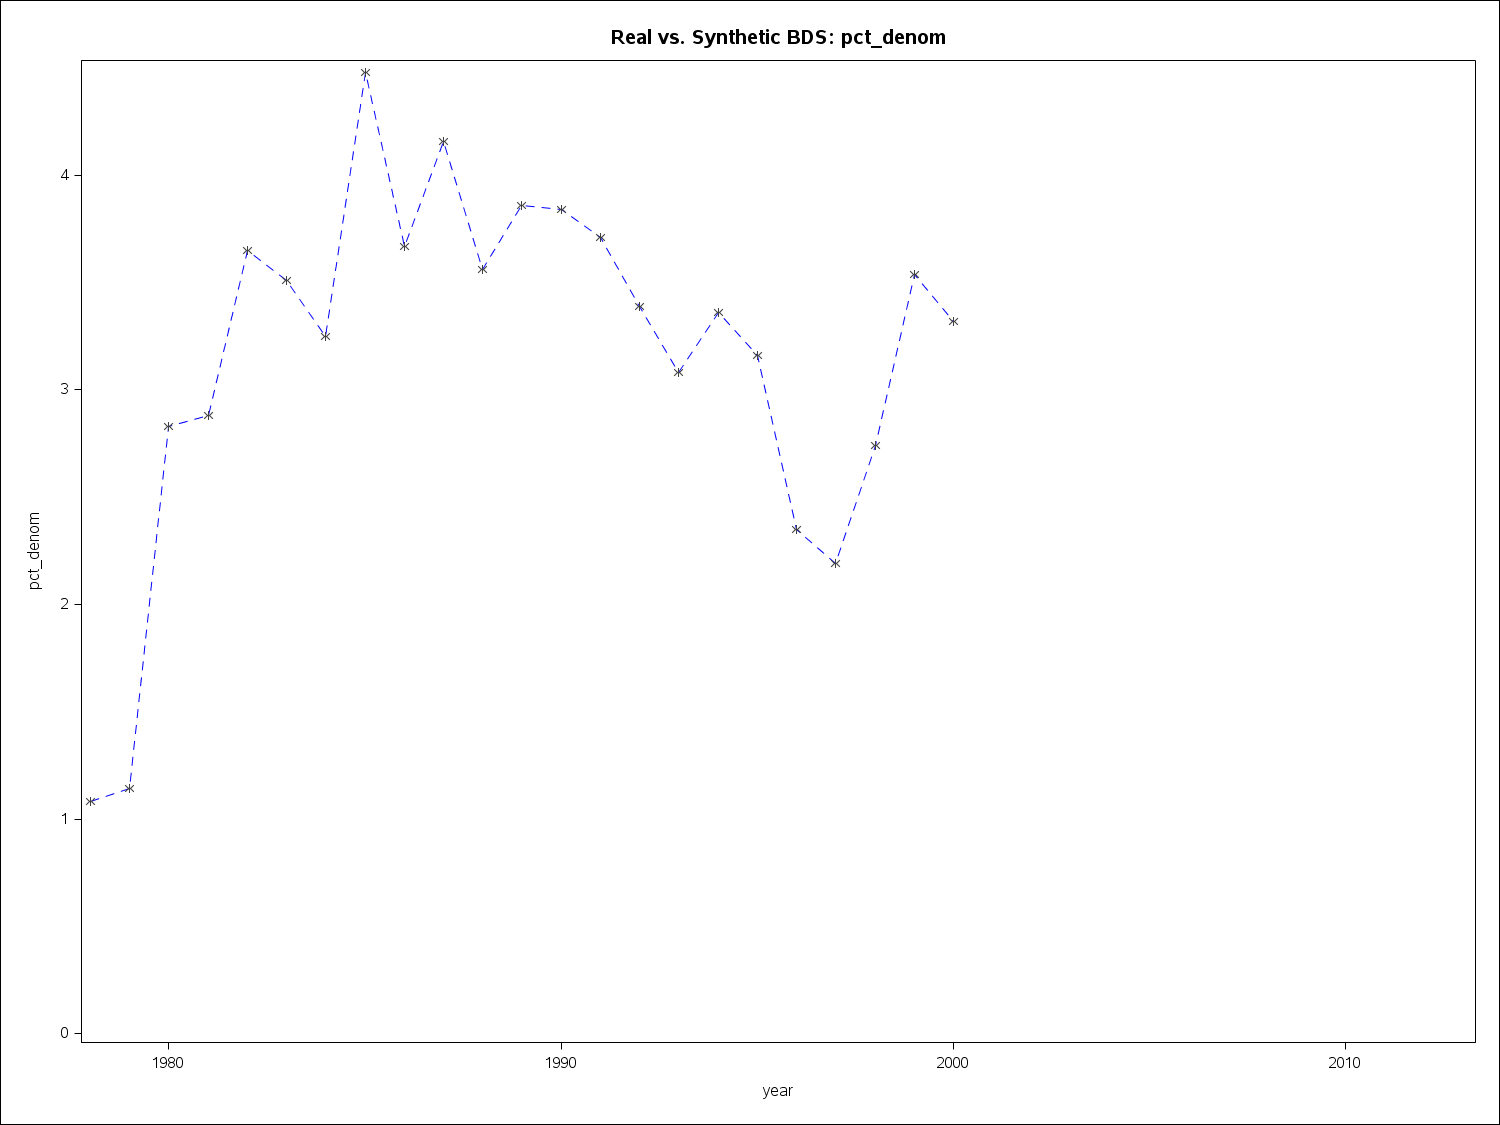
\includegraphics[width=0.45\textwidth]{results/graph_bds_real_vs_syn_pct_denom}
%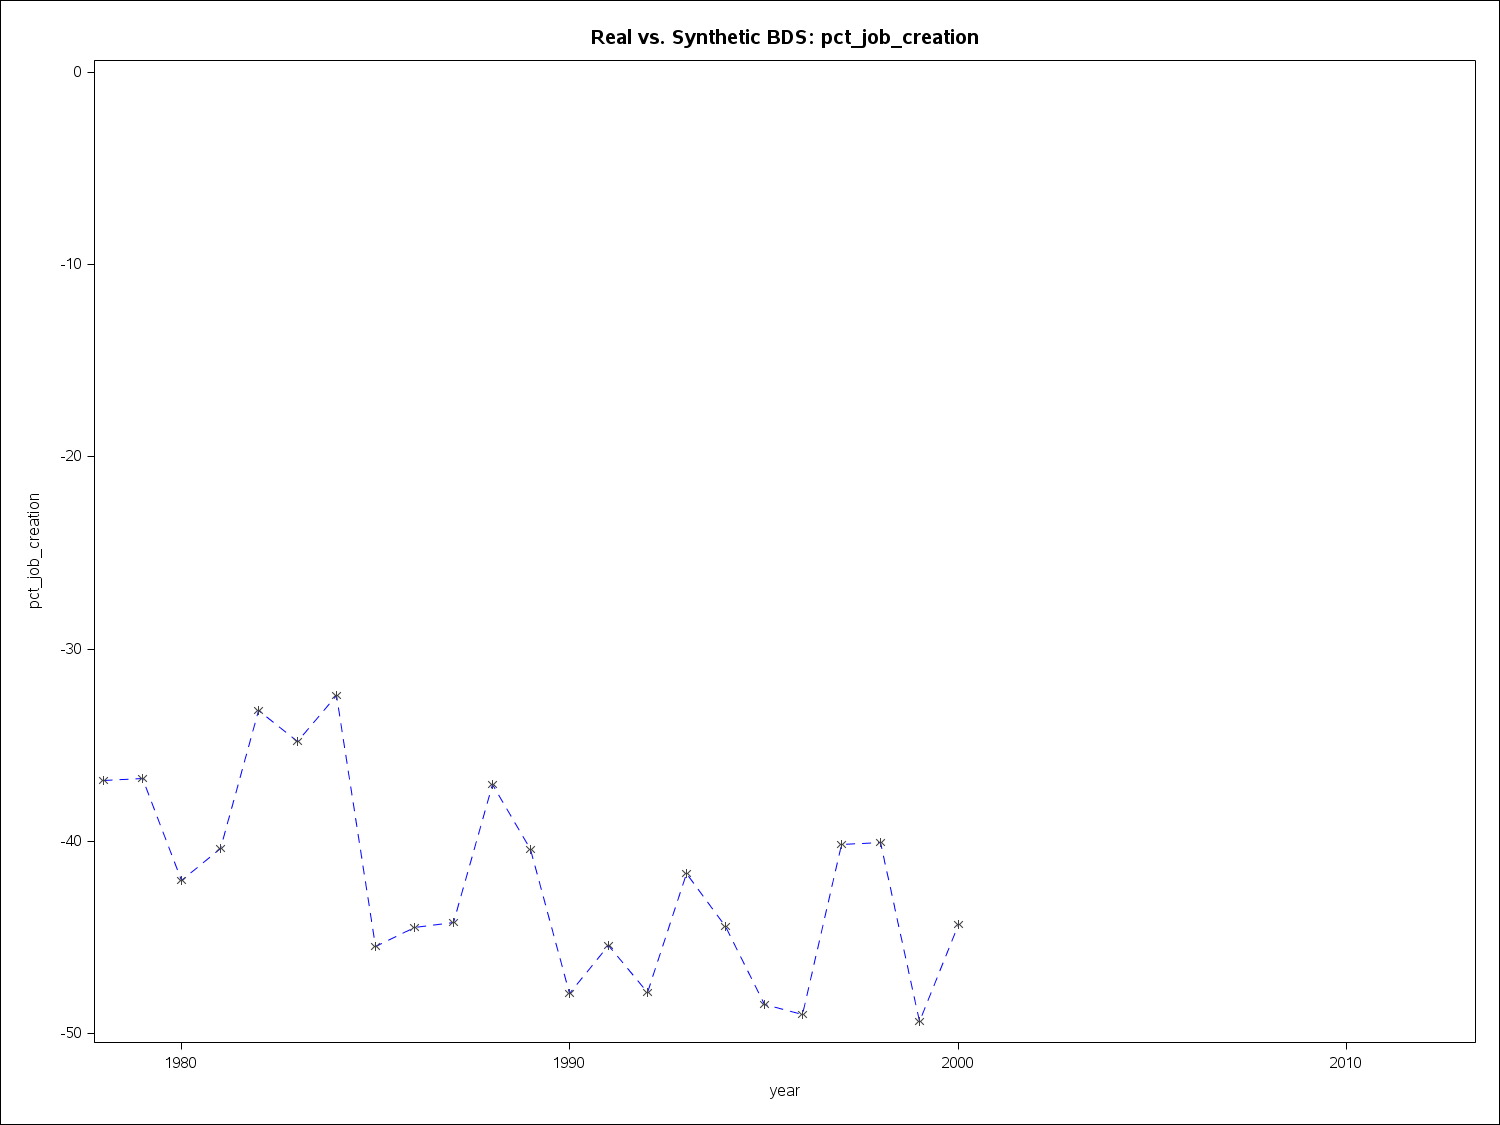
\includegraphics[width=0.45\textwidth]{results/graph_bds_real_vs_syn_pct_job_creation}
%
%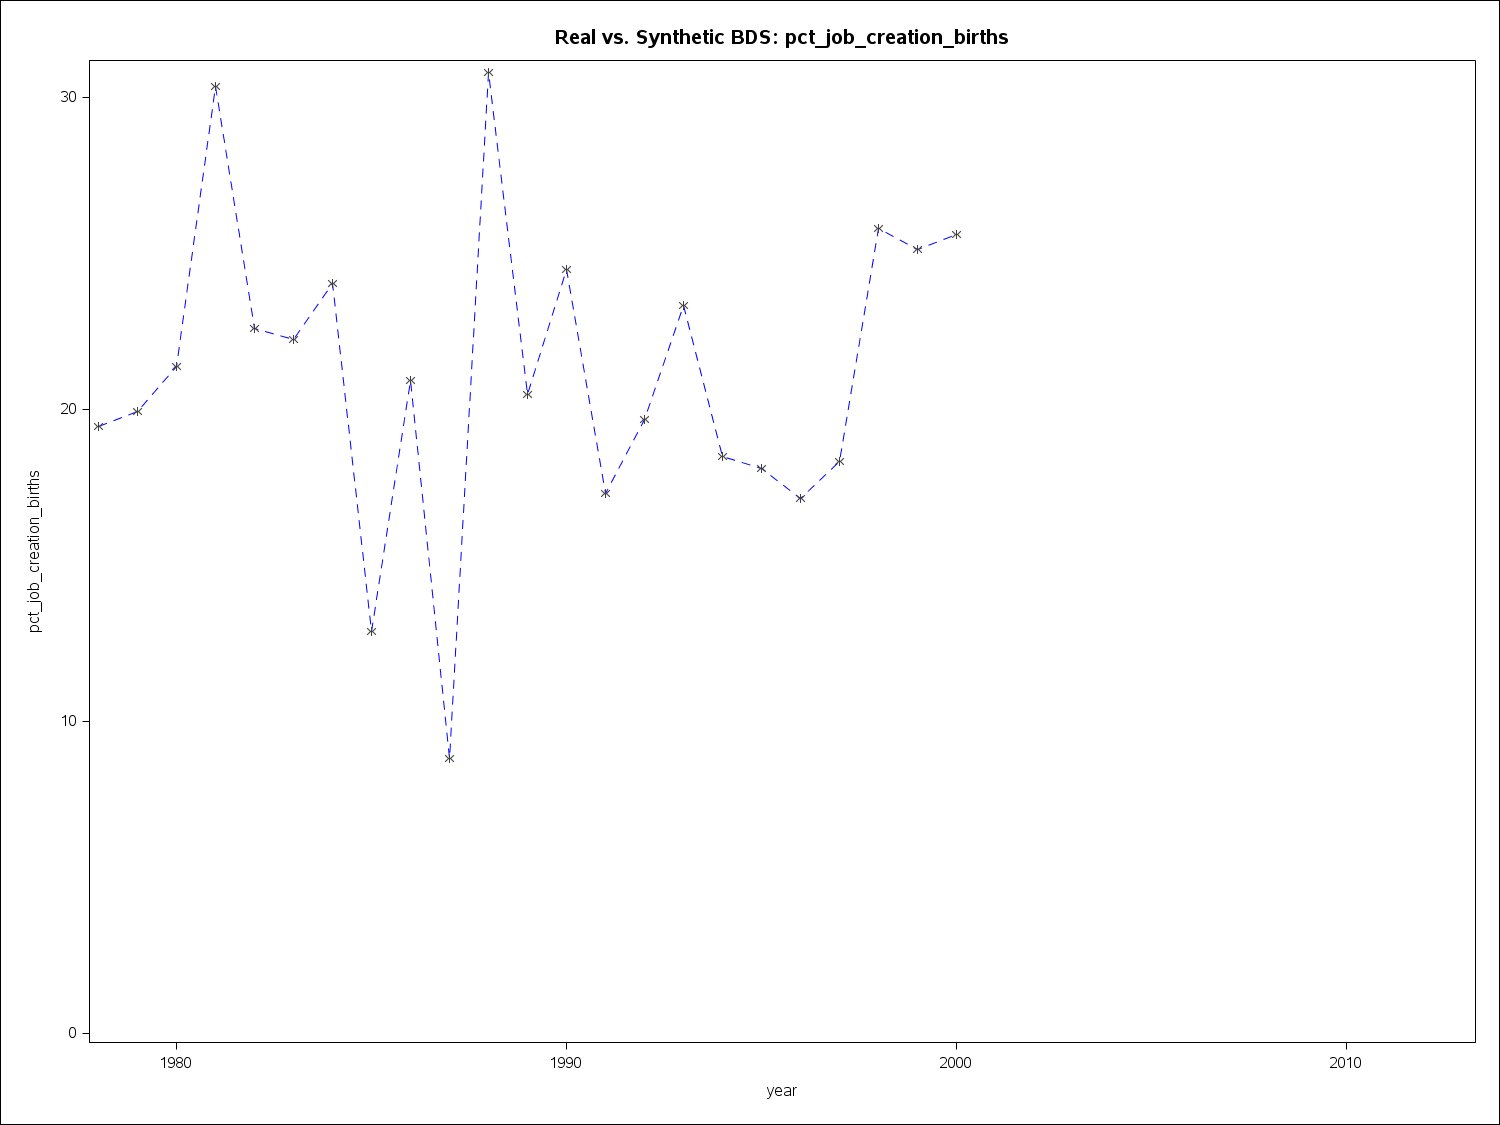
\includegraphics[width=0.45\textwidth]{results/graph_bds_real_vs_syn_pct_job_creation_births}
%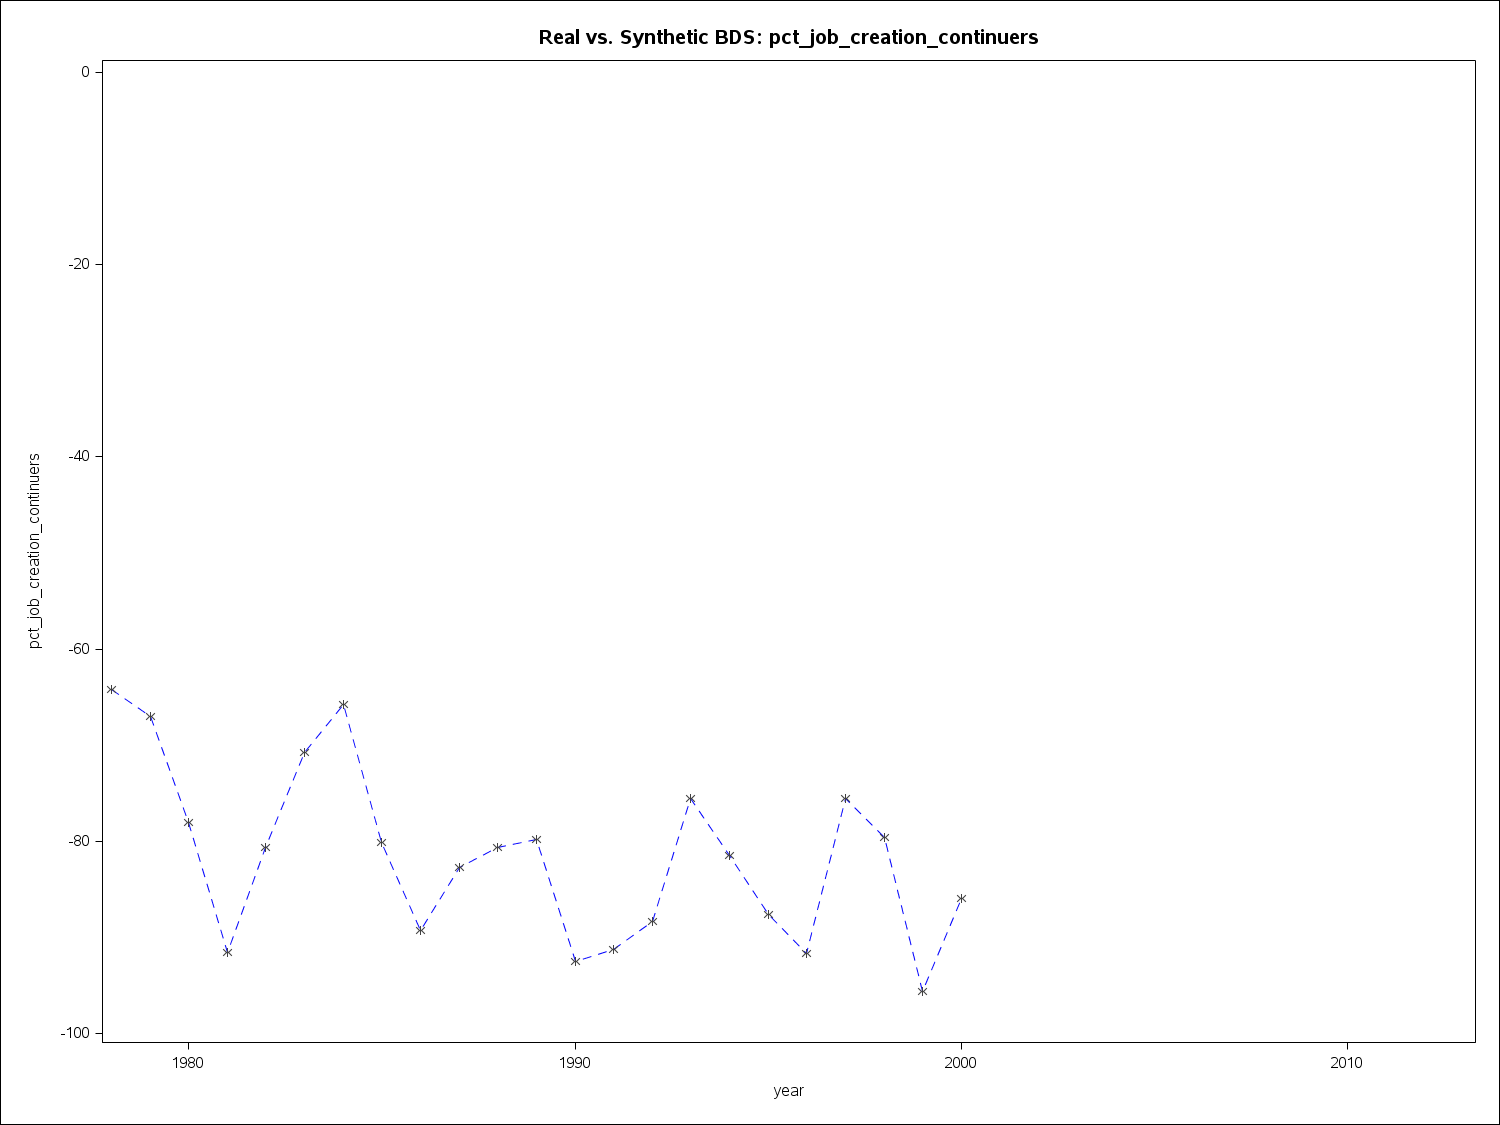
\includegraphics[width=0.45\textwidth]{results/graph_bds_real_vs_syn_pct_job_creation_continuers}
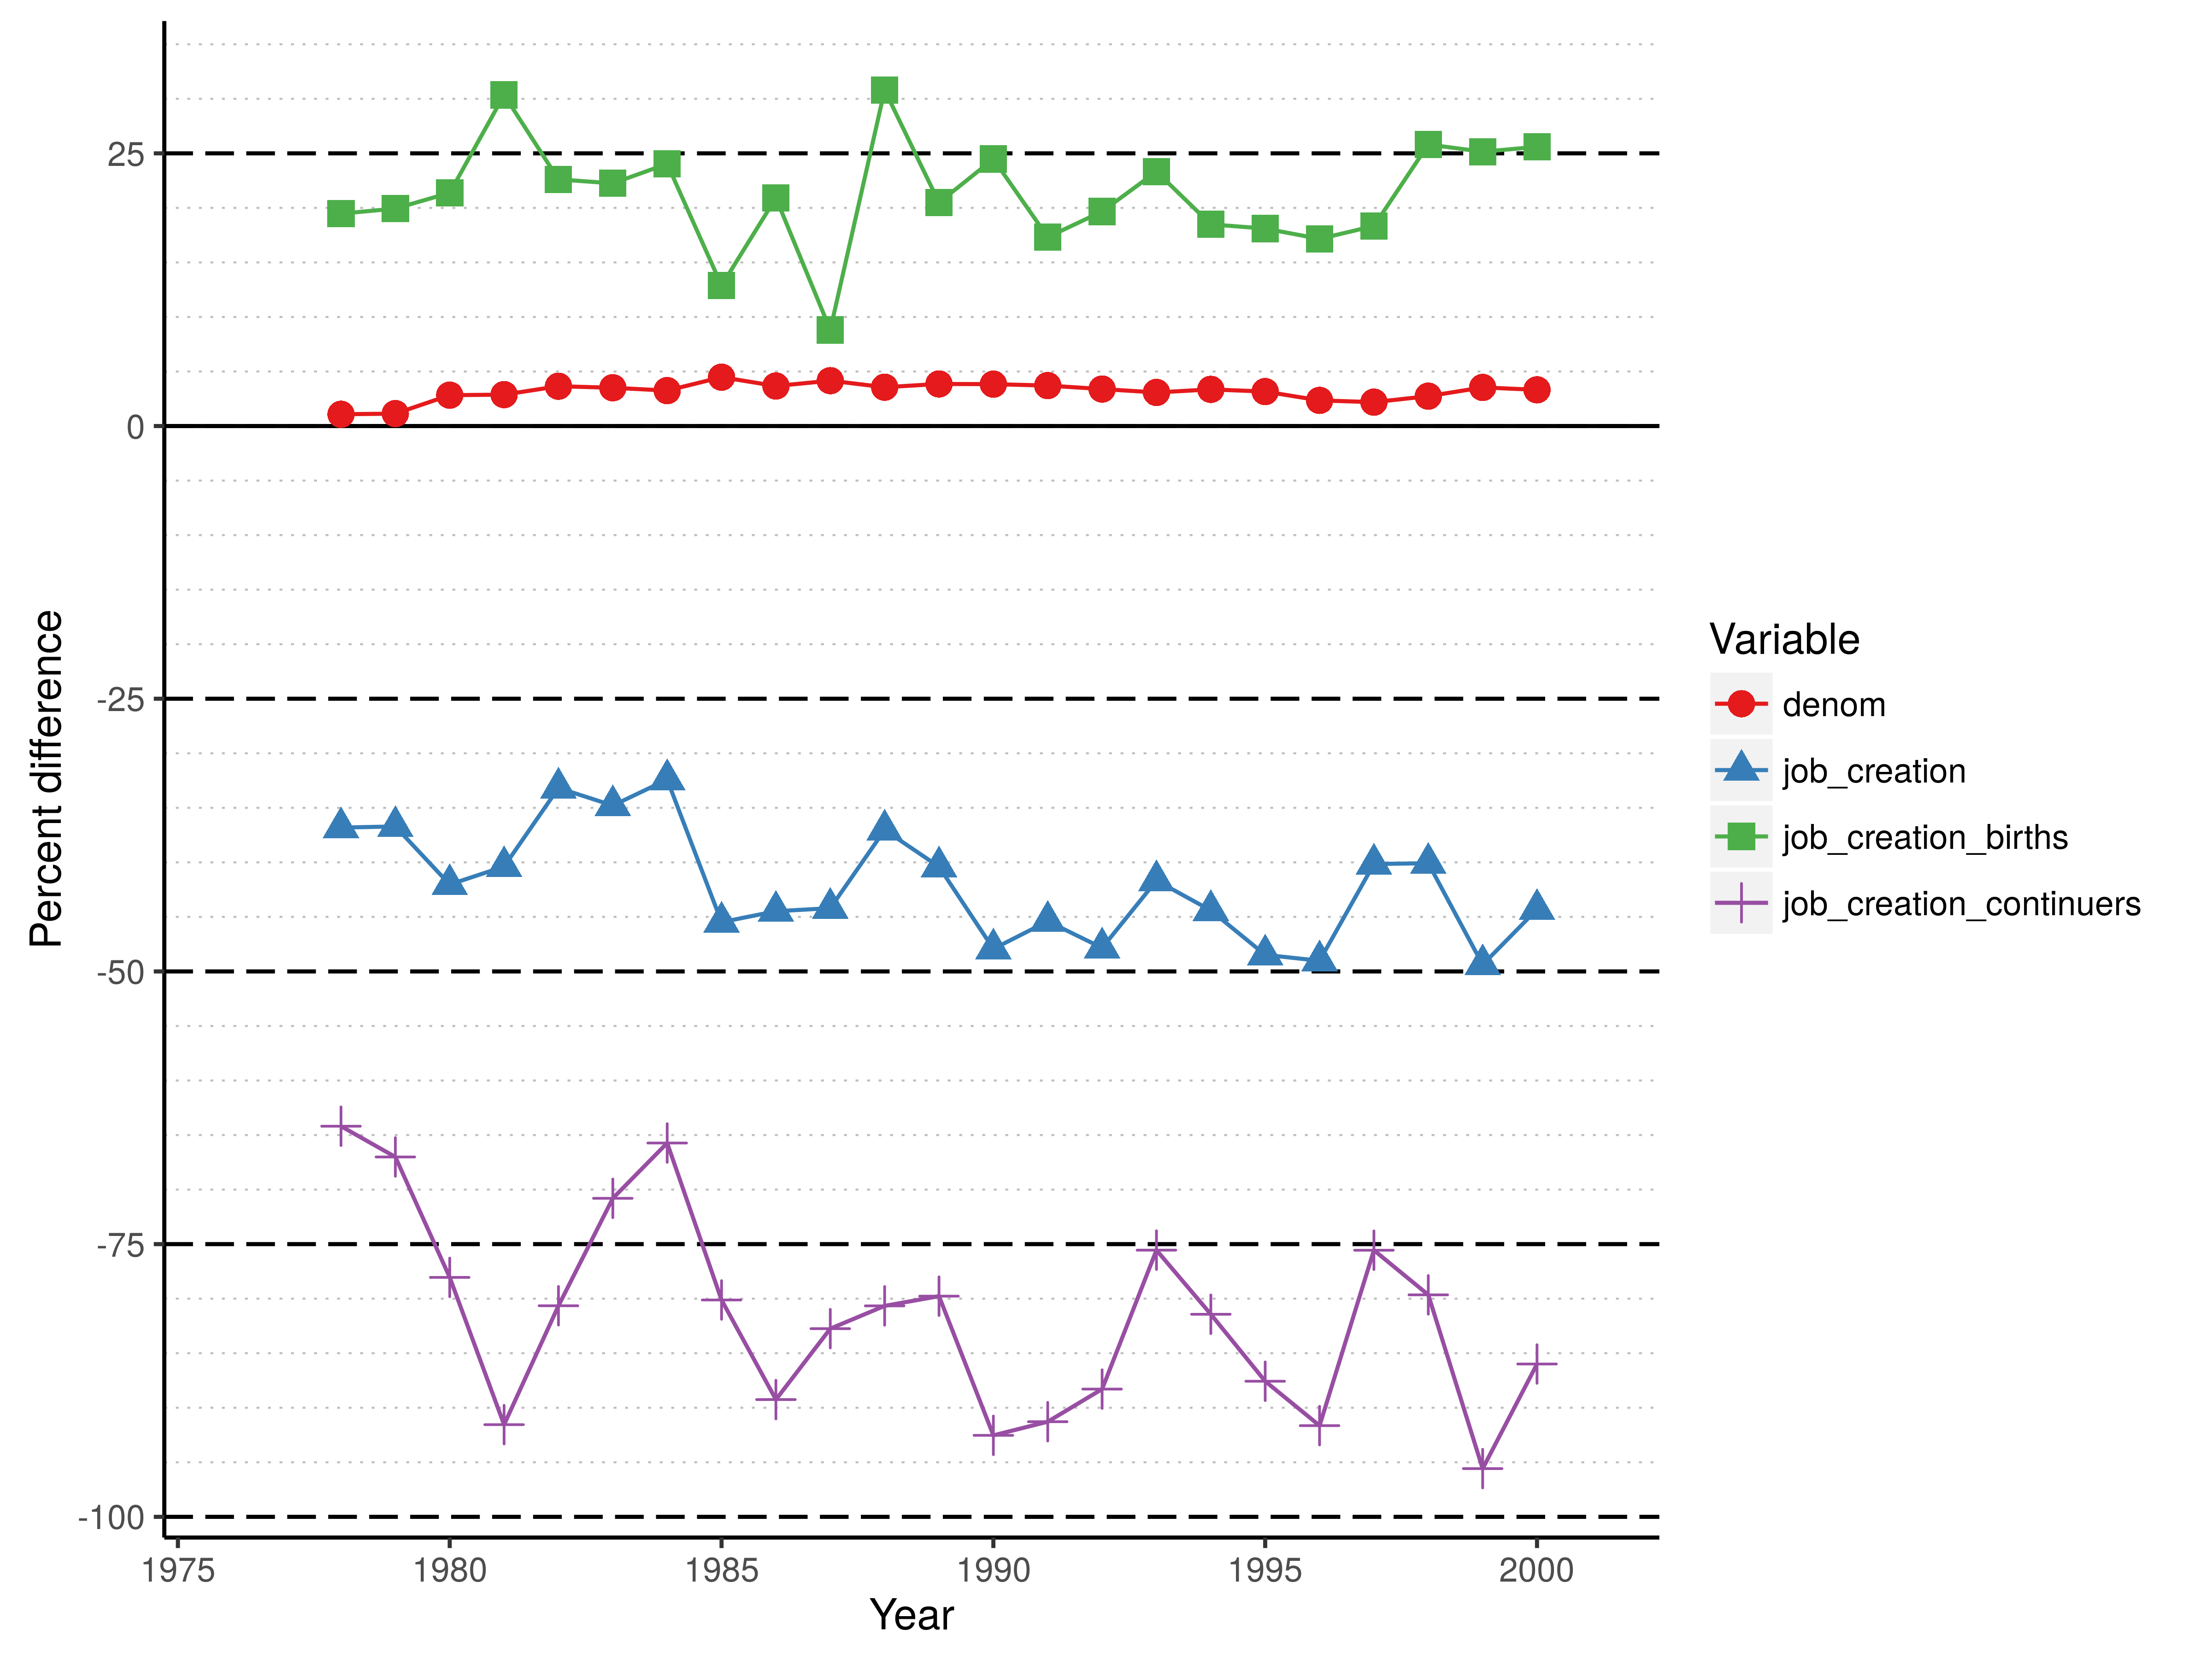
\includegraphics[width=\textwidth]{results/pct_diff_8in}
\end{figure}

